\documentclass[a4paper,12pt]{article}
\usepackage[utf8]{inputenc}
\usepackage{amsmath}
\usepackage{amssymb}
\usepackage{graphicx}
\usepackage{xcolor}
\usepackage{hyperref}
\usepackage{ragged2e}
\usepackage{ngerman}
\usepackage{enumitem}
\usepackage{parskip}

% Farben für Hyperlinks festlegen
\hypersetup{
    colorlinks,
    linkcolor={black},
    citecolor={blue!50!black},
    urlcolor={blue!80!black}
}

\title{Zusammenfassung IT gestützte Geschäftsprozesse}
\author{Student Niclas \& Student Gerrit}
\date{13.07.2024}

\begin{document}
\raggedright

\maketitle
\begin{center}
    {\Large Infos/Änderungsanfragen:} \\[1cm]
    \href{https://github.com/gerritniklas/Zusammenfassung-IT-Geschaeftsprozesse}{GitHub}
\end{center}

\newpage

\tableofcontents

\newpage

\section{Einführung}
\subsection{Betriebliche Informationssysteme}
\begin{itemize}
    \item Unterstützen und koordinieren operative und strategische Geschäftsprozesse. 
    \item Beispiele sind Kundenauftragsprozesse, Produktionsaufträge und Transportaufträge. 
    \item Transaktionsinformationen werden während der Prozesse erfasst, verarbeitet und ausgegeben.
\end{itemize}

\subsection{Managementprozesse}
\begin{itemize}
    \item Informationen werden zur Entscheidungsunterstützung analysiert und verarbeitet.
    \item Beispiele sind Berichte über die Bearbeitungsdauer von Reklamationen und Ablaufplanung von Produktionsaufträgen.
\end{itemize}

\subsection{Daten und Informationen}
\begin{itemize}
    \item Daten sind maschinenlesbare Repräsentationen von Informationen.
    \item Die Nutzung von Daten erfordert Vereinbarungen zur Interpretation.
\end{itemize}

\subsection{Systeme und Schnittstellen}
\begin{itemize}
    \item Ein System besteht aus Komponenten, die miteinander interagieren.
    \item Schnittstellen definieren die Interaktionsmöglichkeiten und den Datenaustausch zwischen Komponenten.
    \item Kommunikationsverbindungen sind für den eigentlichen Datenaustausch verantwortlich.
\end{itemize}

\subsection{Informationssysteme}
\begin{itemize}
    \item Erzeugen, speichern, übertragen und verarbeiten Informationen.
    \item Bestehen aus Menschen und Maschinen und sind sozio-technische Systeme.
    \item Rechnergestützte betriebliche Informationssysteme nutzen Informationstechnologie zur Unterstützung von Geschäftsprozessen.
\end{itemize}

\subsection{Einflussfaktoren}
Änderungen in geschäftlichen Anforderungen, gesetzlichen Vorgaben und technischen Innovationen erfordern kontinuierliche Anpassungen der Informationssysteme.

\subsection{Weitere Informationssysteme}
\begin{itemize}
    \item Persönliche Informationssysteme zur Verwaltung persönlicher Daten.
    \item Zwischenbetriebliche Informationssysteme für den Austausch von Informationen mit Geschäftspartnern und Behörden.
    \item Konsumenteninformationssysteme regeln den Informationsaustausch zwischen Unternehmen und Kunden.
\end{itemize}

\subsection{Technologien}
Beispiele wie RFID zur Identifikation und Lokalisierung von Objekten.

\subsection{Übung}

\subsubsection*{Aufgabe 1.1 (Systembegriff)}
\paragraph*{Aufgabe}
    Bestimmen Sie für die nachstehenden Aussagen, ob diese wahr oder falsch sind. Geben Sie für die als „falsch“ identifizierten Aussagen eine Korrektur an:
    \begin{enumerate}[label=\alph*)]
        \item Die Systemstruktur eines Systems legt fest, wie die Komponenten eines Systems miteinander interagieren.
        \item Als atomar werden Komponenten innerhalb eines Systems bezeichnet, die nicht weiter zerlegt sind.
        \item Die Komponenten eines Systems sind die Elemente des Systems, die nicht miteinander interagieren können.
        \item Die Schnittstelle einer Komponente legt fest, wie mit der Komponente interagiert werden kann.
    \end{enumerate}
\paragraph*{Lösung}
    \begin{enumerate}[label=\alph*)]
        \item Falsch, das Systemverhalten legt fest, wie die Komponenten miteinander kommunizieren können.
        \item Richtig
        \item Falsch, die Komponenten können miteinander kommunizieren
        \item Wahr
    \end{enumerate}

\subsubsection*{Aufgabe 1.2 (Persönliches Informationssystem)}
\paragraph*{Aufgabe}
    Nennen Sie zwei Beispiele, wie Sie durch Ihr persönliches Informationssystem in alltäglichen Tätigkeiten unterstützt werden. Beschreiben Sie dabei, inwiefern das Informationssystem Daten erzeugt, speichert, ausgibt, überträgt und/oder verarbeitet. \\
    Überlegen Sie sich zwei Faktoren, die die kontinuierliche Veränderung Ihres persönlichen Informationssystems beeinflussen und geben Sie jeweils ein Beispiel für die genannten Faktoren an.
\paragraph*{Lösung}
    Beispiel 1: Notizen auf dem Handy, kann von mir angeguckt und ausgelesen werden \\
    Beispiel 2: Smart Home. Eingabe in Handy oder Sprache. Speicherung auf Gerät. Ausgabe: Licht geht an oder eine Szene spielt ab. Übertragung findet über WLAN statt. 
    
    Erweiterung an vorhandene Systeme z.B. kauf eines smarten Kühlschranks, der ins vorhande Smart Home eingebunden wird. \\
    Änderung von System (Architektur). Systeme entwickeln sich weiter bzw. wechselt man eventuell auf einen anderen Hersteller.

\subsubsection*{Aufgabe 1.3 (Betriebliche Informationssysteme)}
\paragraph*{Aufgabe}
    Was ist ein Sozio-Technisches System und warum werden betriebliche Informationssysteme als sozio-technische Systeme bezeichnet. Verdeutlichen Sie ihre Antwort an einem konkreten Beispiel.
\paragraph*{Lösung}
    Ein System, wo Menschen mit einem Computer interagieren müssen, um die Aufgabe zu erfüllen. Bsp. Kassensystem \textrightarrow Mensch tippt Preise ein, System verarbeitet Preise

\subsubsection*{Aufgabe 1.4 (Einflussfaktoren betrieblicher Informationssysteme)}
\paragraph*{Aufgabe}
    Inwiefern hat die Einführung der Bong-Pflicht im Jahr 2020 zu einer Anpassung der Informationssysteme vieler (kleinerer) Unternehmen geführt.
\paragraph*{Lösung}
    Da Sie gezwungen sind jeden Einkauf genau zu dokumentieren, mussten neue Systeme angeschafft bzw. alte Systeme umgebaut werden.

\subsubsection*{Aufgabe 1.5 (Technologien und Konzepte zur Unterstützung von Geschäftsprozessen)}
\paragraph*{Aufgabe}
    Beschreiben Sie für die nachstehend genannten Anwendungsfälle, wie diese durch eine in der Vorlesung vorgestellten Technologien bzw. Konzepte (RFID, Internet der Dinge, virtuelle bzw. erweiterte Realität) sinnvoll unterstützt werden (können).
    \begin{itemize}
        \item Bestellung von Druckertinte
        \item Kauf einer neuen Küche
        \item Rückgabe von ausgeliehenen Werkzeugen (bei einem professionellenWerkzeugverleih)
    \end{itemize}
\paragraph*{Lösung}
    \begin{itemize}
        \item Internet der Dinge \textrightarrow Drucker bestellt Tinte selbst
        \item Virtuelle Realität \textrightarrow Man kann sie die neue Küche genau ansehen, da sie virtuell in das bestehende Zimmer gesetzt wird.
        \item RFID \textrightarrow Chip wird gescannt, und das System erkennt, dass das Gerät zurück gegeben wurde
    \end{itemize}

\subsubsection*{Aufgabe 1.6 (Entscheidungsunterstützung durch Informationsverarbeitung)}
\paragraph*{Aufgabe}
    Sie möchte Ihre Einkaufskosten zur Beschaffung der privaten Lebensmittel reduzieren. Nehmen Sie an, dass Sie die in den vergangenen Jahren Ihre Einkaufslisten konsequent digital gepflegt haben und nun über einen sehr großen Datensatz an Einkaufspositionen verfügen. Der Datensatz umfasst (mindestens) Angaben zu: \\
    Gekauftes Lebensmittel, Einkaufspreis, Geschäft (in dem gekauft wurde) \\
    Wie könnten Sie diese Informationen verwenden, um Ihre Einkaufskosten ggf. zukünftig zu reduzieren?
\paragraph*{Lösung}
    Vergleich der Preise von gleichen Produkten in verschiedenen Läden. So kann man den günstigsten Preis finden.





\section{Geschäftsprozessmanagement}

\subsection{Grundlagen zu Geschäftsprozessen}
    \subsubsection*{Definition}
        Geschäftsprozesse sind die arbeitsteilige Ausführung von Aktivitäten in einer zeitlich-/sachlogischen Reihenfolge zur Erfüllung einer betrieblichen Aufgabe.
    \subsubsection*{Sichten}
        \begin{itemize}
            \item Steuerungssicht: Darstellung des Ablaufs eines Prozesses. Identifikation der Ereignisse (durch die ein Prozess ausgelöst wird bzw. die ein Prozess auslöst).
            \item Funktionssicht: Beschreibung und Zerlegung der Funktionen, die innerhalb eines Prozesses ausgeführt werden.
            \item Datensicht: Beschreibt Daten, die benötigt werden bzw. erzeugt werden.
            \item Organisationssicht: Beschreibt duch wen die Funktionen ausgeführt werden (z.B. Meschen oder Maschienen).
            \item Leistungssicht: Beschreibt die durch die Ausführung des Prozesses entstehenden Mehrwerte/Wertschöpfungen.
        \end{itemize}
    \subsubsection*{Arten}
        Wertschöpfende Kernprozesse, unterstützende Prozesse, Management Prozesse.
    \subsubsection*{Prozesstyp vs. Prozessinstanz}
        Typ ist die Vorlage, Instanz die konkrete Ausführung.

\subsection{Merkmale und Lebenszyklus des Geschäftsprozessmanagements}
    \subsubsection*{Ziele}
        Prozesse effektiver und effizienter gestalten.
    \subsubsection*{Rollen}
        \begin{itemize}
            \item Geschäftsführung: Verantwortlich für die grundsätzliche Gestaltung der Geschäftsprozesse.
            \item Prozessverantwortlicher: Verantwortlich für die Ausführung und Anpassung der Prozesse.
            \item Prozessteilnehmer: Führen Routineaufgaben innerhalb der Prozesse aus.
            \item Systemanalytiker: Erhebt, analysiert und verbessert Prozesse.
            \item Anwendungsentwickler: Verantwortlich für die softwaretechnische Umsetzung.
        \end{itemize}
    \subsubsection*{Lebenszyklus}
        \begin{figure}[h]
            \centering
            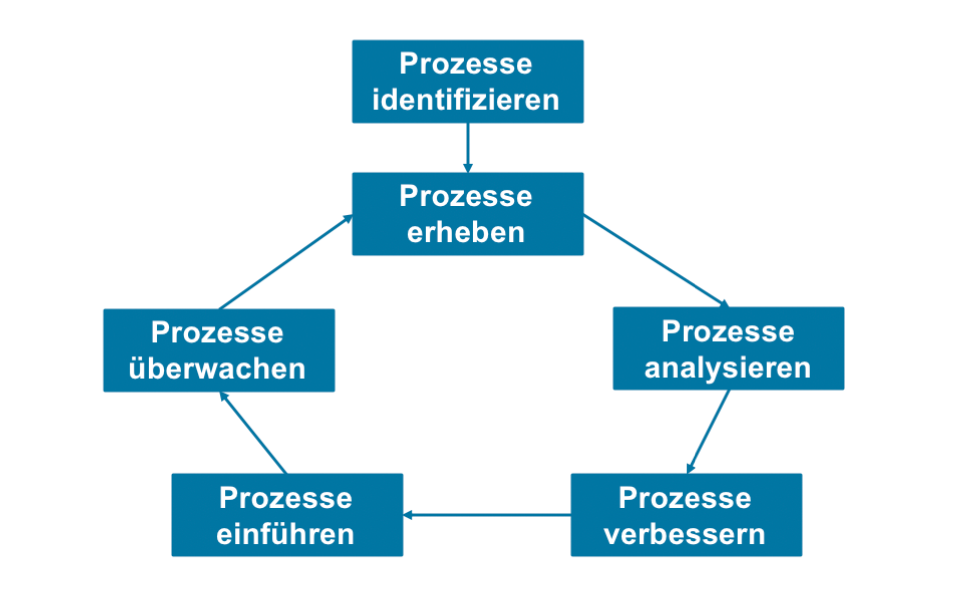
\includegraphics[width=\textwidth]{image/Lebenszyklus.png}
            \caption{Lebenszyklus Geschäftsprozessmanagements}
            \label{fig:Lebenszyklus}
        \end{figure}

\subsection{Identifikation von Geschäftsprozessen}
    \subsubsection*{Vorgehen}
        Erfassung der wichtigsten Prozesse, Darstellung als Prozesslandkarte oder Wertschöpfungskette, Bewertung und Auswahl der zu verbessernden Prozessen.
    \subsubsection*{Referenzmodelle}
        Dienen als Vorlagen zur Entwicklung spezifischer Prozesse. Bespiel: Handels-H-Modell (Abbildung \ref{fig:Handels-H-Modell}). Anerkannte Lösung für wiederkehrende Probleme.
        \begin{figure}[h]
            \centering
            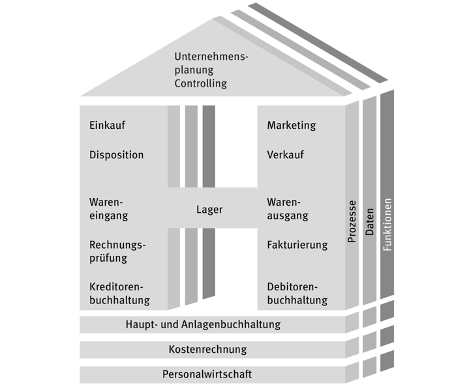
\includegraphics[width=\textwidth]{image/Handels-H-Modell.png}
            \caption{Handels H Modell}
            \label{fig:Handels-H-Modell}
        \end{figure}
    \subsubsection*{Techniken}
        Prozessmodellierung und -analyse zur Optimierung.

\subsection{Gestaltung von Geschäftsprozessen}
    \subsubsection{Prozesse erheben}
        \paragraph*{Ziel}
            Sammeln von Informationen über den aktuellen Ablauf eines Prozesses (IST-Modell).
        \paragraph*{Methoden}
            \begin{itemize}
                \item Dokumentensichtung: Nutzt vorhandene Dokumente, kann aber veraltet sein.
                \item Beobachtung: Direkte Erkennung des IST-Zustands, jedoch zeitaufwendig.
                \item Interviews: Detaillierte Informationen, aber zeitintensiv.
                \item Workshops: Kompakte und kollaborative Erhebung, jedoch zeitaufwendig für alle.
            \end{itemize}

    \subsubsection{Prozesse analysieren}
        \paragraph*{Ziel}
            Identifizieren von Schwachstellen und deren Ursachen.
        \paragraph*{Typische Schwachstellen}
            \begin{itemize}
                \item Lange Durchlaufzeiten
                \item Hohe Fehlerquote
                \item Hohe Kosten
                \item Geringe Flexibilität
            \end{itemize}
        \paragraph*{Methoden}
            \begin{itemize}
                \item Qualitative Analyse: Wertbeitragsanalyse, Ursache-Wirkungsdiagramme.
                \item Quantitative Analyse: Nutzung statistischer Daten zur Identifikation von Engpässen.
            \end{itemize}

    \subsubsection{Prozesse verbessern}
        \paragraph*{Ziel}
            Vorschläge zur Eliminierung von Schwachstellen und Erstellung eines SOLL-Prozesses.
        \paragraph*{Dimensionen der Verbesserung}
            Durchlaufzeit, Kosten, Qualität, Flexibilität. (Abbildung \ref{fig:Teufelsviereck})
            \begin{figure}[ht]
                \centering
                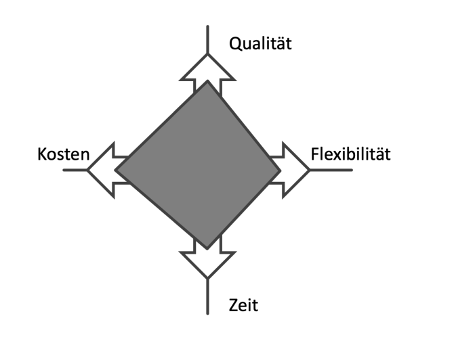
\includegraphics[width=\textwidth]{image/Teufelsviereck.png}
                \caption{Teufelsviereck}
                \label{fig:Teufelsviereck}
            \end{figure}
        \paragraph*{Methoden}
            \begin{itemize}
                \item Verbesserungsvorschläge in den genannten Dimensionen erarbeiten.
                \item Redesign-Heuristiken: Konkrete Maßnahmen zur Umgestaltung von Prozessen.
            \end{itemize}

\subsection{Ausführung von Geschäftsprozessen}
    \subsubsection*{Umsetzung}
        Prozesse in die Praxis umsetzen durch Implementierung und Anpassung von Anwendungssystemen.
    \subsubsection*{Beispiele}
        Implementierung neuer Systeme, Anpassung bestehender Systeme, Bereitstellung benötigter Geräte.

\subsection{Prozesse einführen}
    \subsubsection*{Definition}
        Organisatorische und technische Maßnahmen zur Bereitstellung der Infrastruktur.
    \subsubsection*{Maßnahmen}
        Mitarbeiterschulung, Schaffung neuer Stellen, Anpassung bestehender Stellen, Implementierung oder Anpassung von Anwendungssystemen.

\subsection{Prozesse überwachen}
    \subsubsection*{Prozessüberwachung}
        Überwachung anhand aufgezeichneter Daten.
    \subsubsection*{KPI (Key Performance Indicators)}
        Aggregation und Darstellung von Kennzahlen zur Überwachung und Identifikation von Optimierungspotentialen.
\subsection{Übung}

\subsubsection*{Aufgabe 2.1 (Effektiv vs. Effizient)}
\paragraph*{Aufgabe}
    Bewerten Sie, ob der nachfolgend beschriebene Prozess (aus dem persönlichen Umfeld) effektiv und effizient ist. Beachten Sie bei der Bewertung insb. die nachstehende Beobachtung. 

    Prozess: Lebensmittel einkaufen 
    \begin{itemize}
        \item Schritt 1: Einkaufsliste (Lebensmittel) schreiben 
        \item Schritt 2: Lebensmittelgeschäft auswählen
        \item Schritt 3: Zum Lebensmittelgeschäft fahren
        \item Schritt 4: Produkte gemäß Einkaufsliste auswählen 
        \item Schritt 5: Bezahlen 
        \item Schritt 6: Produkte verladen
        \item Schritt 7: Produkte nach Hause transportieren und in Schränke einräumen 
    \end{itemize}

    Beobachtung: Im Schritt 4 besuchen Sie die einzelnen Abteilungen (z.B. Obst, Reinigungsmittel) des Lebensmittelgeschäfts häufiger, da immer wieder noch ein Produkt aus der jeweiligen Abteilung fehlt. 

\paragraph*{Lösung}
    Nein, da einzelne Abteilungen immer mehrfach besucht werden, das wiederum braucht Zeit. Um das zu beheben sollte man die Lebensmittel nach Abteilung sortieren.
    Man sollte außerdem noch Preise pro Lebensmittelgeschäft vergleichen und das günstigste Lebensmittelgeschäft raussuchen.

\subsubsection*{Aufgabe 2.2 (Rollen im Geschäftsprozessmanagements)}
\paragraph*{Aufgabe}
    \begin{enumerate}[label=\alph*)]
        \item Beschreiben Sie die Aufgaben, die der Rolle des „Prozessverantwortlichen“ im Rahmen des Geschäftsprozessmanagement zukommen.
        \item Welche weiteren Rollen sind für das Geschäftsprozessmanagement relevant?
    \end{enumerate}
   
\paragraph*{Lösung}
    \begin{enumerate}[label=\alph*)]
        \item Verantwortlich für die Ausführung und Anpassung der Prozesse
        \item Geschäftsführung, Prozessteilnehme, Systemanalytiker, Anwendungsentwickler
    \end{enumerate}

\subsubsection*{Aufgabe 2.3 (Prozessverbesserung)}
\paragraph*{Aufgabe}
    Wie könnte das in Aufgabe 2.1 beobachtete Problem, das zur Verschwendung von Zeitressourcen führt, durch eine bessere Strukturierung der Einkaufsliste behoben werden?
   
\paragraph*{Lösung}
    In dem man die Lebensmittel auf der Einkaufsliste nach Abteilungen sortiert

\subsubsection*{Aufgabe 2.4 (Sichten auf Prozesse)}
\paragraph*{Aufgabe}
    \begin{enumerate}[label=\alph*)]
        \item Welche Sichten werden bei der Darstellung von Prozessen unterschieden? Beschreiben Sie die genannten Sichten kurz.
        \item Beschreiben Sie im Kontext der Datensicht, welche Informationen eine Einkaufsliste (vgl. Aufgabe 2.1) enthalten sollte und wie diese Informationen strukturiert sein sollten, um das in Aufgabe 2.1 identifizierte Problem zu beseitigen.
        \item Welche Informationen müssen zur Erstellung einer in Teilaufgabe b) beschriebenen Einkaufsliste im Vorfeld vorliegen?
    \end{enumerate}
   
\paragraph*{Lösung}
    \begin{enumerate}[label=\alph*)]
        \item Sichten:
        \begin{itemize}
            \item Steuerungssicht: Darstellung des Ablaufs eines Prozesses. Identifikation der Ereignisse (durch die ein Prozess ausgelöst wird bzw. die ein Prozess auslöst).
            \item Funktionssicht: Beschreibung und Zerlegung der Funktionen, die innerhalb eines Prozesses ausgeführt werden.
            \item Datensicht: Beschreibt Daten, die benötigt werden bzw. erzeugt werden.
            \item Organisationssicht: Beschreibt duch wen die Funktionen ausgeführt werden (z.B. Meschen oder Maschienen).
            \item Leistungssicht: Beschreibt die durch die Ausführung des Prozesses entstehenden Mehrwerte/Wertschöpfungen.
        \end{itemize}
        \item Name, Preis, Anzahl, Abteilung. Das sollte in einer Tabelle dargestellt werden.
        \item Alle aufgelisteten Informationen.
    \end{enumerate}


\subsubsection*{Aufgabe 2.5 (Lebenszyklus des Geschäftsprozessmanagements)}
\paragraph*{Aufgabe}
    \begin{enumerate}[label=\alph*)]
        \item Welche Phasen werden im Lebenszyklus des Geschäftsprozessmanagements unterschieden?
        \item Zu welcher Phase des Lebenszyklus sind die in Aufgabe 2.4b durchgeführten Schritte zuzuordnen?
    \end{enumerate}
   
\paragraph*{Lösung}
    \begin{enumerate}[label=\alph*)]
        \item Prozesse indentifizieren, Prozesse erheben, Prozesse analysieren, Prozesse verbessern, Prozesse einführen, Prozesse überwachen.
        \item Prozesse überwachen, da wir dort Daten zur Ausführung der Prozesse sammeln und analysieren.
    \end{enumerate}


\subsubsection*{Aufgabe 2.6 (Prozessidentifikation)}
\paragraph*{Aufgabe}
    Identifizieren Sie die Prozesse die in einem typischen Prüfungsamt (z.B. im SSB der FH SWF) ausgeführt werden bzw. an denen ein typisches Prüfungsamt beteiligt ist und stellen Sie diese in Form einer selbst gewählten Prozesslandkarte dar.
   
\paragraph*{Lösung}
    Fragen beantworten \textrightarrow fördert \textrightarrow Immatrikulation


\subsubsection*{Aufgabe 3.1 (Dimensionen zur Prozessverbesserung)}
\paragraph*{Aufgabe}
    \begin{itemize}
        \item Aktivität 1 (Warenwirtschaftssystem): Druckt Pickliste zum Kundenauftrag aus.
        \item Aktivität 2 (Mitarbeiter 1 - Hilfsmittel Einkaufskorb): Stellt die Waren manuell gemäß der Pickliste zusammen und bringt diese in den Kommissionierbereich.
        \item Aktivität 3 (Mitarbeiter 2): Prüft die Vollständigkeit der vom Mitarbeiter 1 kommissionierten Produkte nach Art und Anzahl.
        \item Aktivität 4 (Mitarbeiter 2): Verpackt die kommissionierten Waren und klebt das Versandetikett (Lieferadresse, Route) auf die Verpackung.
        \item Aktivität 5 (Mitarbeiter 3): Bringt das Paket aus dem Kommissionierbereich in den Warenausgangsbereich.
        \item Aktivität 6 (Mitarbeiter 4): Der Mitarbeiter 4 entnimmt das Paket aus dem Warenausgangsbereich und liefert es mit dem Lieferwagen an die auf dem Versandetikett hinterlegte Adresse
    \end{itemize}

    Versetzen Sie sich in folgende Situation: Die Kunden beschweren sich in letzter Zeit zunehmend darüber, dass sie abgelaufene Lebensmittel erhalten.

    Bearbeiten Sie die folgenden Aufgaben:
    \begin{enumerate}[label=\alph*)]
        \item Auf welche Dimension der Geschäftsprozessverbesserung bezieht sich die Beschwerde der Kunden?
        \item Entwickeln Sie einen (möglichst einfachen) Vorschlag zur Anpassung des Prozesses, um die Belieferung von Kunden mit abgelaufenen Lebensmitteln zu vermeiden oder zu reduzieren.
        \item Verdeutlichen Sie die Bedeutung des „Teufelsviereck des Geschäftsprozessmanagements“ an Ihrem Beispiel.
    \end{enumerate}
\paragraph*{Lösung}
    \begin{enumerate}[label=\alph*)]
        \item Qualität.
        \item Der Mitarbeiter 1, der die Pickliste zusammenstellt, prüft währenddessen ob die Lebensmittel, die er in den Warenkorb packt noch halbar sind.
        \item Wenn sich die Qualität verbessern, hat man automatisch einbußen bei Kosten, Flexibilität und Zeit. Das heißt mehr Kosten, weniger Flexibilität und mehr Zeit.
    \end{enumerate}


\subsubsection*{Aufgabe 3.2 (Redesign Heuristiken)}
\paragraph*{Aufgabe}
    Lesen Sie die Erläuterung zu den Heuristiken im Lehrbuch auf den Seiten 118 - 120 und machen Sie einen Vorschlag (inkl. Begründung!) welche Heuristik Sie in den folgenden Situationen anwenden würden, um die beschriebenen Probleme zu lösen bzw. zu verringern:
    
    \begin{enumerate}[label=\alph*)]
        \item Ein Produktentwicklungsprozess (im Individualmaschinenbau) wird durch häufiges Nachfragen der Entwickler beim Kunden stark verzögert (u.a., weil immer wieder auf die Antworten des Kunden gewartet werden muss).
        \item Beim Verkaufsprozess eines Automobilhändlers werden häufig Ressourcen verschwendet, da mehrere Prozessschritte von den Mitarbeitern bereits ausgeführt werden (Abschlussinspektion durchführen, Fahrzeug reinigen, Anmeldung vorbereiten), bevor das Ergebnis der Kreditwürdigkeitsprüfung vorliegt.
        \item Bei der Störungsbearbeitung eines Telekommunikationsunternehmens kommt es zu längeren Bearbeitungszeiten, weil die Mitarbeiter während der Ausführung einer Prozessinstanz immer wieder wechseln und die neuen Mitarbeiter sich erneut in den Gegenstand der Störung einarbeiten müssen.
        \item Bei der regelmäßigen Bestellung von Rohstoffen bei einem Lieferanten wird die vom Lieferanten erhaltene Rechnung per Hand in das Buchhaltungssystem übernommen. Neben der dafür erforderlichen Zeit kommt es auch häufig zu Fehler bei der Übernahme der Rechnungsdaten.
    \end{enumerate}

\paragraph*{Lösung}
    \begin{enumerate}[label=\alph*)]
        \item Kontaktreduktion
        \item Änderung der Abfolge
        \item Zusammenfassung
        \item Automatisierung, Kontrolle
    \end{enumerate}

\subsubsection*{Aufgabe 3.3 (Analyse von Prozessen)}
\paragraph*{Aufgabe}
    Sie stellen (subjektiv) fest, dass Sie häufig bestimmte Lebensmittel nicht im Haus haben, die Sie eigentlich benötigen. Analysieren Sie Ihren (einen hypothetischen) Einkaufsprozess mit dem Ursachen-Wirkungs-Diagramm auf mögliche Ursachen für diese Beobachtung.
\paragraph*{Lösung}
    Keine Lösung


\subsubsection*{Aufgabe 3.4 (Einführung von Prozessen)}
\paragraph*{Aufgabe}
    Versetzen Sie sich in folgende Situation: Sie möchten den Einkaufsprozess in Ihrem familiären Umfeld bzw. in Ihrer Haushaltsgemeinschaft durch die Nutzung einer Einkaufslisten-App verbessern. Das SOLL-Modell zum Prozess ist bereits entwickelt worden:
   
    \begin{itemize}
        \item Schritt 1: Haushaltsmitglieder tragen Ihre Einkaufswünsche in die App ein.
        \item Schritt 2 (immer Mittwochs): Die App erstellt aus den Einkaufswünschen der Haushaltsmitglieder eine gesammelte Einkaufsliste und sortiert diese gemäß des Aufbaus des ausgewählten Lebensmittelgeschäfts)
        \item Schritt 3: Die mit dem Einkaufen beauftragte Personen fährt zum Lebensmittelgeschäft und führt den Einkauf gemäß der Einkaufsliste durch.
        \item Schritt 4: Die eingekauften Produkte werden in die dafür vorgesehenen Schränke eingeräumt.
    \end{itemize}

    Welche Maßnahmen müssen zur Einführung des SOLL-Modell ergriffen werden?
\paragraph*{Lösung}
    Geräte bereitstellen, Personen an den Geräten schulen, App implementieren, Personen an der App schulen, Person zum einkaufen bestimmen.



\section{Modellierung betrieblicher Informationssysteme}

\subsection{Grundlagen der Modellierung}
    \subsubsection*{Definition und Ziele}
        Die Modellierung dient der konsistenten, korrekten und vollständigen Erfassung und Darstellung der Anforderungen an betriebliche Informationssysteme. Ziel ist es, Geschäftsprozesse und unterstützende betriebliche Anwendungen optimal aufeinander abzustimmen.
    \subsubsection*{Charakteristika}
        Ein Modell ist eine vereinfachte und zweckorientierte Abbildung eines realen oder imaginären Sachverhalts.
        \begin{itemize}
            \item Abbildungscharakter: Sicht auf bestimmten Bezugspunkt
            \item Vereinfachung: Modell ist immer „einfacher“ als eigentlicher Sachverhalt
            \item Zweckorientierung: Modell hat immer einen bestimmten Zweck
        \end{itemize}
    \subsubsection*{Prinzipien/Eigenschaften}
        \begin{itemize}
            \item Partitionierung: Zerlegung eines komplexen Sachverhalts in isolierte Teilbereiche
            \item Projektion: Betrachtung eines Sachverhalts aus verschiedenen Perspektiven
            \item Abstraktion: Vernachlässigung unwesentlicher Details zur Fokussierung auf wesentliche Aspekte
        \end{itemize}
    \subsubsection*{Arten von Modellen}
        \begin{itemize}
            \item IST-Modell: Zeigt den aktuellen Zustand (dokumentierend)
            \item SOLL-Modell: Zeigt den geplanten zukünftigen Zustand (entwerfend)
            \item Referenzmodell: Anerkannte Lösungsvorschlag, dient zum Vergleich mit IST und als Vorlage für SOLL
        \end{itemize}

\subsection{Modellierungssprachen}
    \subsubsection*{Definition}
        Modellierungssprachen definieren die Syntax und Semantik für die Erstellung von Modellen.
    \subsubsection*{Beispiele}
        BPMN (Business Process Model and Notation) verwendet spezifische Symbole und Regeln zur Darstellung von Geschäftsprozessen.
    \subsubsection*{Ausdrucksstärke}
        Die Ausdrucksstärke einer Modellierungssprache bestimmt, welche Aspekte eines Sachverhalts dargestellt werden können und wie detailliert diese sind.

\subsection{Grundzüge ordnungsgemäßer Modellierung}
    \subsubsection*{Richtigkeit}
        Modelle müssen den zu modellierender Sachverhalt korrekt abbilden (semantisch und syntaktisch).
    \subsubsection*{Relevanz}
        Modelle sollten alle relevanten Details enthalten und irrelevante Details ausblenden.
    \subsubsection*{Wirtschaftlichkeit}
        Relevante Details sollten nur modelliert werden, wenn deren Erhebung nicht zu aufwendig ist.
    \subsubsection*{Klarheit}
        Modelle müssen verständlich dargestellt werden.
    \subsubsection*{Vergleichbarkeit}
        Vergleichbarkeit: Einheitliche Terminologie und Struktur für Modelle eines Unternehmens.
    \subsubsection*{Systematik}
        Modelle müssen systematisch organisiert sein.

\subsection{Architektur Integrierter Informationssysteme (ARIS)}
    \subsubsection*{Definition}
        ARIS beschreibt die ganzheitliche Struktur eines Unternehmens in Form der verwendeten Prozesse, Organisationsstrukturen, Funktionen, Daten und Kommunikationsbeziehungen.
    \subsubsection*{Ziele}
        Reduktion der Komplexität durch Rahmenwerke wie ARIS, um eine systematische und einheitliche Modellierung zu ermöglichen.
    \begin{figure}[h]
        \centering
        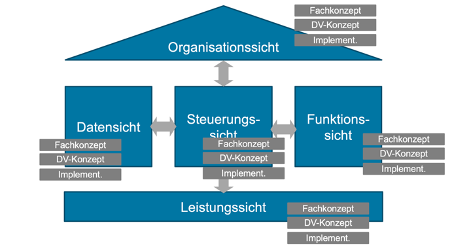
\includegraphics[width=\textwidth]{image/ARIS.png}
        \caption{ARIS}
        \label{fig:ARIS}
    \end{figure}

\section{Modellierung von Geschäftsprozessen}

\subsection{Grundlagen zur Geschäftsprozessmodellierung}
    \subsubsection*{Eigenschaften von Prozessmodellen}
        Modelle bilden reale oder imaginäre Sachverhalte ab und sind abstrahiert, um relevante Details für den jeweiligen Verwendungszweck zu erfassen.
    \subsubsection*{Verwendungszwecke}
        Organisatorische Anwendungsfälle (Verständnis, Kommunikation, Analyse, Verbesserung, Weiterentwicklung) und Systementwicklung (Vorlage für Softwaresysteme, z.B. Workflow-Engine)

\subsection{Einfache Prozessmodelle}
    \subsubsection*{Grundlegende Elemente}
        \begin{itemize}
            \item Aktivitäten: aus einzelschritten gebündelte Arbeitseinheit (z.B. Rechnung erstellen)
            \item Ereignis: tritt spontan auf (z.B. Kunde storniert Auftrag)
            \item Sequenzfluss: Ereignisse und Aktivitäten stehen in logischer Beziehung
            \item Startereignis: Bestimmt wann eine Prozessinstanz gestartet wird
            \item Endereignis: Bestimmt wann eine Prozessinstanz beendet, wird
        \end{itemize}
    \subsubsection*{Marken}
    Zeigen den aktuellen Schritt einer Prozessinstanz und dienen der Analyse

\subsection{Verzweigungen und Parallelisierungen}
    \subsubsection*{Exklusive ODER}
        Hier Bild
    \subsubsection*{Parallelisierung}
        Hier Bild
    \subsubsection*{Inklusiv Oder}
        Hier Bild

\subsection{Geschäftsobjekte und Ressourcen}
    \subsubsection*{Geschäftsobjekte}
        Elemente, die innerhalb eines Prozesses verwendet oder erstellt werden. 
        \begin{itemize}
            \item Erstellen eines Angebots -> erzeugt Angebot -> Angebot versenden. 
            \item Symbol: Datei. Werden mit - - - - > Aktivitäten verbunden.
        \end{itemize}
    \subsubsection*{Ressourcen}
        Menschen, Maschinen und Materialien, die zur Durchführung von Aktivitäten benötigt werden. 
        \begin{itemize}
            \item Werden durch Bahnen dargestellt.
            \item Aktivitäten werden den Ressourcen zugeordnet.
        \end{itemize}

\subsection{Prozesszerlegung}
    \subsubsection*{Hierarchische Strukturierung}
        Zerlegung komplexer Prozesse in kleinere, handhabbare Subprozesse (Fragmente) zur besseren Übersicht und Steuerung.
    \subsubsection*{Modularisierung}
        Bildung von Modulen, die unabhängig voneinander entwickelt und gewartet werden können.

\subsection{Ereignisse und Behandlung von Ausnahmen}
    \subsubsection*{Zwischenereignisse}
        Bild (doppelter Rand)
    \subsubsection*{Ausnahmen}
        Bild (Blitz)

\section{Analyse von Geschäftsprozessen}

\subsection{Ziele und Methoden der Prozessanalyse}
    \subsubsection*{Ziele}
        Das systematische Aufspüren von Schwachstellen und Verbesserungspotentialen zur kontinuierlichen Verbesserung der Prozesse.
    \subsubsection*{Methoden}
        Unterscheidung zwischen qualitativen und quantitativen Analyseansätzen. Qualitative Methoden umfassen eine methodische Vorgehensweise zur Problemerkennung, während quantitative Methoden analytisch vorgehen und auf Rechenwerken basieren.

\subsection{Wertschöpfungsanalyse}
    Kunden eines Prozesses sind jene die einen Vorteil durch die Ausführung einen Prozess haben (interne oder externe Kunden eines Prozesses)
    \subsubsection*{Zerlegung der Aktivitäten}
        Aktivitäten eines Prozesses in Schritte unterteilen, danach bewerten (Wertschöpfend, Geschäftsförderlich, nicht-Wertschöpfend)
    \subsubsection*{Eliminierung ineffizienter Schritte}
        Nicht-wertschöpfende Schritte sollen eliminiert oder automatisiert werden

\subsection{Ursachen-Wirkungsdiagramm}
    \begin{figure}[ht]
        \centering
        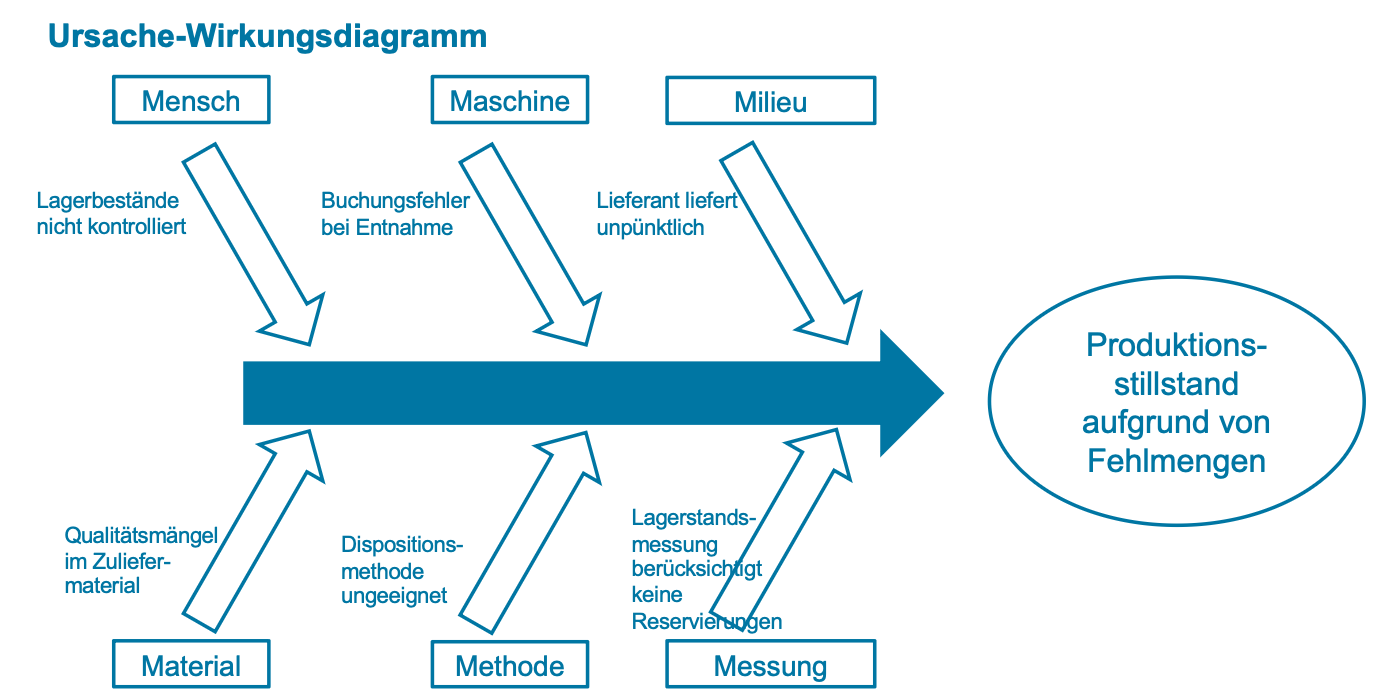
\includegraphics[width=\textwidth]{image/Ursachen-Wirkungsdiagramm.png}
        \caption{Ursachen-Wirkungsdiagramm}
        \label{fig:Ursachen-Wirkungsdiagramm}
    \end{figure}
    \subsubsection*{6M-Methode}
        Identifikation von Ursachen für Prozessprobleme in den Kategorien Mensch, Maschine, Milieu (Prozessumfeld), Material, Methode (Konzeption) und Messung (Daten)
    \subsubsection*{Diagrammerstellung}
        Dokumentation und Klassifizierung der Ursachen in Haupt- und Nebenursachen zur Vorbereitung von Diskussionen

\subsection{Durchlaufzeitanalyse}
    \subsubsection*{Ziel}
        Bewertung der durchschnittlichen Bearbeitungszeit einer Prozessinstanz
    \subsubsection*{Sequenz von Aktivitäten}
        \begin{itemize}
            \item Formel: $DZ_{\text{Sequenz}} = \sum T_i$
            \item Beispiel: Wenn die Durchlaufzeit der Aktivitäten T1, T2 und T3 jeweils 2, 3, 5 Stunden betragen, dann $2+3+5=10$ Stunden
        \end{itemize}
    \subsubsection*{XOR-Block}
        \begin{itemize}
            \item Formel: $DZ_{\text{XOR}} = \sum (p_i * T_i)$
            \item Beispiel: Wenn es zwei Pfade gibt, einer mit einer Wahrscheinlichkeit von 20\% und einer Dauer von 30 Stunden und der andere mit einer Wahrscheinlichkeit von 80\% und einer Dauer von 40 Stunden, dann ist die durchschnittliche Durchlaufzeit $0.2*30+0.8*40=6+32=40$ Stunden
        \end{itemize}
    \subsubsection*{UND-Block}
        \begin{itemize}
            \item Formel: $DZ_{\text{UND}} = T_{\text{parallel}} + max(T_1, T_2, ...)$
            \item Beispiel: Wenn eine parallele Aktivität 10 Stunden dauert und zwei parallele Sequenzflüsse 20 Stunden bzw. 30 Stunden benötigen, dann ist die durchschnittliche Durchlaufzeit $10+max(20, 30)=10+30=40$ Stunden
        \end{itemize}
    \subsubsection*{Wiederholung}
        \begin{itemize}
            \item Formel: $DZ_{\text{Loop}} = \frac{T_{\text{Loop}}}{1-p}$
            \item Beispiel: Angenommen, die Durchlaufzeit für eine Aktivität innerhalb der Schleife beträgt 5 Stunden und die Wahrscheinlichkeit, dass die Schleife wiederholt wird, ist 30\% (also p = 0.3), dann ist die durchschnittliche Durchlaufzeit $\frac{5}{1-0.3}=\frac{5}{0.7} \approx 7,14$ Stunden
        \end{itemize}
    \subsubsection*{Durchlaufzeiteffizienz (DLE)}
        \begin{itemize}
            \item Formel: $DLE = \frac{Bearbeitungszeit}{\text{Gesamte Durchlaufzeit}}$
            \item Beispiel: Wenn die Bearbeitungszeit eines Prozesses 4 Stunden beträgt und die gesamte Durchlaufzeit 10 Stunden ist, dann berechnet sich die Durchlaufzeiteffizienz wie folgt: $DLE= \frac{4 Stunden}{10 Stunden}=40\%$
        \end{itemize}

\section{Datenmodellierung}

\subsection{Ziel der ER-Modelle}
    \begin{itemize}
        \item Darstellung der im betrieblichen Informationssystem relevanten Daten.
        \item Visualisierung der Datenobjekte (Entitäten) mit ihren Attributen und den Beziehungen zwischen ihnen auf Typebene.
    \end{itemize}

\subsection{Modellelemente von ER-Modellen}
    \subsubsection*{Entitäten}
        \begin{itemize}
            \item Identifizierbare und abgrenzbare Datenobjekte (z.B. Kunde, Rechnung)
            \item Besitzen Attribute und Beziehungen zu andren Entitäten
            \item Darstellung durch Rechtecke
        \end{itemize}
    \subsubsection*{Attribute}
        \begin{itemize}
            \item Relevante Eigenschaften einer Entität (z.B. Name, Rechnungsbetrag)
            \item Schlüsselattribute (identifizieren die Entitäten eindeutig) werden unterstrichen
            \item Darstellung durch Ovale
        \end{itemize}
    \subsubsection*{Relationen}
        \begin{itemize}
            \item Beziehungen zwischen Entitäten (z.B. Kunde <-> Rechnung)
            \item Darstellung durch Rauten, die mit den in Beziehungen stehenden Entitäten verbunden werden
        \end{itemize}

\subsection{Kardinalitäsverhältnisse}
    \begin{itemize}
        \item Beschreiben die Anzahl der Entitäten, die an einer Beziehung teilnehmen können.
        \item 1:1-Beziehung: Eine Entität ist mit genau einer anderen Entität verbunden
        \item 1:n-Beziehung: Eine Entität der ersten Art mit mehreren Entitäten der zweiten Art verbunden, aber jede Entität der zweiten Art nur mit einer der ersten Art
        \item n:n-Beziehung: Entitäten beider Art können beliebig oft miteinander in Beziehung stehen
    \end{itemize}

\section{Betriebliche Anwendungssysteme}

\subsection{Definition und Klassifikation betrieblicher Anwendungen}
    \subsubsection*{Definition}
        Betriebliche Anwendungssysteme sind Softwarelösungen, die zur Unterstützung und Optimierung von Geschäftsprozessen in Unternehmen dienen.
    \subsubsection*{Klassifikation}
        Sie werden in verschiedene Kategorien eingeteilt, wie z.B. Transaktionssysteme, Planungssysteme, und Kontrollsysteme.
    \subsubsection*{Integration}
        Horizontale Integration (Funktionsbereichsübergreifend) und vertikale Integration (überunterschiedliche Managementebenen hinweg) sind wesentliche Aspekte.

\subsection{ERP-Systeme (Enterprise-Resource-Planning)}
    \subsubsection*{Funktion}
        ERP-Systeme sind integrierte Anwendungssysteme, die zur Planung und Steuerung der unternehmensweiten Ressourcen eingesetzt werden. Zu den verwalteten Ressourcen gehören Materialien, Personal, Finanzmittel und mehr.
    \subsubsection*{Integration}
        ERP-Systeme bieten sowohl horizontale als auch vertikale Integration. Horizontale Integration unterstützt operative Geschäftsprozesse in verschiedenen Funktionsbereichen. Vertikale Integration ermöglicht analytische Funktionen zur Berichterstellung und Entscheidungsunterstützung.
    \subsubsection*{End-to-End-Prozesse}
        ERP-Systeme unterstützen durchgehende Prozesse wie den Order-to-Cash und Procure-to-Pay-Prozess ohne Medienbrüche.

\subsection{Standard- vs. Individualsoftware}
    \subsubsection*{Standardsoftware}
        Software, die von einem Hersteller für den Einsatz in vielen verschiedenen Unternehmen entwickelt wird. Sie bietet eine breite Funktionalität und hohe Qualität, erfordert jedoch Anpassungen für spezifische Geschäftsprozesse.
        \begin{itemize}
            \item Vorteile: Höhere Qualität, umfangreiche Funktionen, kontinuierliche Weiterentwicklung.
            \item Nachteile: Geringe Abbildung individueller Prozesse, Abhängigkeit vom Hersteller, hoher Einführungsaufwand.
        \end{itemize}
    \subsubsection*{Individualsoftware}
        Speziell für die Bedürfnisse eines einzelnen Unternehmens entwickelt. Sie bietet maßgeschneiderte Lösungen, kann aber teurer und aufwändiger in der Entwicklung sein.
    \subsubsection*{Anpassungen}
        Standardsoftware kann durch Customizing, Erweiterungsprogrammierung und Modifikation an spezifische Anforderungen angepasst werden. Release Fähigkeit: Alte individuelle Anpassungen sind nach dem Einspielen des nächsten Releases automatisch wieder verfügbar

\subsection{Einführung von ERP-Systemen}
    \subsubsection*{Chancen}
        Verbesserte Prozessstandardisierung, zentrale Datenspeicherung und Integration von Unternehmensprozessen.
    \subsubsection*{Risiken}
        Fehlende Nutzung aller Funktionen, Unterschätzung des Einführungsaufwands, Schwierigkeiten bei der Datenmigration und hohen Kosten durch Softwareanpassungen.
    \subsubsection*{Dienstleister}
        Oft übernehmen externe Dienstleister den Betrieb der ERP-Systeme, wobei die Leistungen in Service-Level-Agreements festgehalten sind.
    \subsubsection*{Vorgehensmodell}
        \begin{itemize}
            \item Initialisierung \& Situationsanalyse
            \item Entwicklung des Sollkonzepts
            \item Marktanalyse
            \item Systemauswahl
            \item Realisierung
            \item Einführung \& Betrieb
        \end{itemize}

\subsection{Anwendungslandschaften}
    \subsubsection*{Definition}
        Die Gesamtheit der in einer Organisation betriebenen betrieblichen Anwendungen und deren Verbindungen.
    \subsubsection*{Entwicklung}
        Früher monolithische Systeme mit Medienbrüchen, heute service-orientierte Architekturen mit standardisierten Schnittstellen für eine nahtlose Integration.
    \subsubsection*{Integration}
        Moderne Anwendungslandschaften ermöglichen eine softwaretechnische Integration ohne Medienbrüche.

\section{E-Commerce}

\subsection{Grundlagen eCommerce}
    \subsubsection*{Definition}
        Abwicklung von Markttransaktionen unter Verwendung von Internet-Technologien
    \subsubsection*{Ziel}
        Prozesse mit externen Akteuren effektiver und effizienter zu gestalten
    \subsubsection*{Markttransaktionsphasen}
        \begin{itemize}
            \item Informationsphase: Beschaffung von Informationen (Suchkosten)
            \item Vereinbarungsphase: Aushandlung der Zahlungs- und Lieferkonditionen, Übermittlung der erforderlichen Daten, Abschluss des Kaufvertrags.
            \item Abwicklungsphase: Austausch der vereinbarten Leistung (Transportkosten, Überweisungskosten)
        \end{itemize}
    \subsubsection*{Transaktionskosten}
        Kosten, die in den verschiedenen Phasen der Ausführung einer Markttransaktion anfallen.
    \subsubsection*{Unterscheidung nach Geschäftspartner} 
        \begin{itemize}
            \item Business 2 Business (B2B): Zwischenbetriebliche Interaktion
            \item Business 2 Customer (B2C): Absatz von Produkten und Dienstleistungen an Endkunden
            \item Business 2 Government (B2G): Geschäftsbeziehung zwischen Unternehmen und der öffentlichen Verwaltung
            \item Customer 2 Customer (C2C): Handel von Produkten zwischen Endkunden
        \end{itemize}

\subsection{Zwischenbetriebliche Informationssysteme (B2B/B2G)}
    \subsubsection*{Definition}
        Unterstützung der elektronischen Abwicklung von Geschäftsprozessen zwischen verschiedenen Unternehmen und zwischen Unternehmen und der öffentlichen Verwaltung.
    \subsubsection*{Aufgabe}
        Austausch von Informationen zwischen Akteuren durch gemeinsame Kommunikationsbeziehungen und Vereinbarungen zur Interpretation der Daten.
    \subsubsection*{Standards}
        EDIFACT (Electronic Data Interchange for Administration, Commerce and Transport) ist ein Internationaler Standard zur Strukturierung von Dokumenten zwischenbetrieblichen Austausch von Informationen. Dieser Umfasst über 200 Nachrichtentypen (Rechnungen, Bestellungen, Produktstammdaten)

\subsection{Außenwirksame Informationssysteme}
    \subsubsection*{Definition}
        Systeme, die sich an externe Anwender richten (Kunden, Geschäftskunden, Lieferanten, Dienstleister, Behörden) und die IT-gestütze Abwicklungen von unternehmensübergreifenden Geschäftsprozessen ermöglichen
    \subsubsection*{Klassifikation}
        \begin{itemize}
            \item Unterstützte Funktionsbereiche
            \item Unterstützte Prozessebene
            \item Produkt- und Branchenorientierung
            \item Unterstütze Markttransaktionsphasen
            \item Adressierte Zielgruppen
            \item Konzeptionelle Ausrichtung
            \item IS-Betreiber
        \end{itemize}

\subsection{Spezielle außenwirksame Informationssysteme}
    \subsubsection*{Unternehmensinformationsportale}
        \begin{itemize}
            \item Bieten externen Benutzern (Kunden, Lieferanten) Zugriff auf Informationen über das Unternehmen und Produkte
            \item Bieten Informationen eines internen Informationssystems für angemeldete Benutzer (z.B. Lagerbestand)
        \end{itemize}
    \subsubsection*{eShops}
        Darstellung/Verkauf von Produkten/Dienstleistungen \\
        Unterstützung der Transaktionsphasen:
        \begin{itemize}
            \item Informationsphase: Detaillierte Produktdarstellung.
            \item Vereinbarungsphase: Bestimmung Zahlungs- und Lieferbedingungen.
            \item Abwicklungsphase: Zahlungsabwicklung.
        \end{itemize}
    \subsubsection*{Lieferantenprotale}
        \begin{itemize}
            \item Integration von Lieferanten in die Informationsverarbeitung.
            \item Unterstützung des Einkaufprozesses durch Bereitstellung von Produktkatalogen und Abwicklung der Bestellungen.
        \end{itemize}

\subsection{Internetdienste im Zusammenhang des E-Commerce}
    \subsubsection*{Suchdienste}
        Ermöglichen die Suche nach bestimmten Inhalten (Webseiten, Produkten, Dienstleistungen) im Internet
    \subsubsection*{Klassifikationen}
        \begin{itemize}
            \item Gegenstand der Suche: Objekte, Personen, Produkte, Dienstleistungen
            \item Bereich der Suche: Internetdienste, begrenzter Raum (unternehmen, regional), medienbezogen (Text, Ton, Bild, Video)
            \item Verfahren der Suche: Indexbasierte Stichwortsuche, indexbasierte Volltextsuche, semantische Suche
        \end{itemize}

\end{document}